% Borg GPU — HPG 2026 Poster
% A0 landscape, tikzposter

\documentclass[a0paper,landscape,25pt]{tikzposter}

% ── Theme ──────────────────────────────────────────────────────────────────
\usetheme{Rays}
\usecolorstyle{Spain}   % dark blue + orange accent; swap as desired

% ── Packages ───────────────────────────────────────────────────────────────
\usepackage[utf8]{inputenc}
\usepackage[T1]{fontenc}
\usepackage{lmodern}
\usepackage{booktabs}
\usepackage{graphicx}
\usepackage{tikz}
\usetikzlibrary{positioning}
\usepackage{amsmath,amssymb}
\usepackage{xcolor}
\usepackage{enumitem}
\newcommand{\todo}[1]{\textcolor{red}{[#1]}}

% ── Custom colours ─────────────────────────────────────────────────────────
\definecolor{borgblue}{HTML}{1A3C5E}
\definecolor{borgorange}{HTML}{E87722}
\definecolor{borggreen}{HTML}{2E7D32}

% ── Custom block style ─────────────────────────────────────────────────────
\newcommand{\done}{\textcolor{borggreen}{$\checkmark$}}
\newcommand{\inprog}{\textcolor{borgorange}{\textbf{[wip]}}}

% ── Title ──────────────────────────────────────────────────────────────────
\title{\textbf{Borg}: A Complete Open-Source TBDR GPU Pipeline\\
       with ASIC Tapeout on 5280 Logic Cells}
\author{Andreas Wendleder}
\institute{Independent Researcher, Landshut, Germany
           \quad \texttt{andreas.wendleder@proton.me}
           \quad \texttt{github.com/gonsolo/Borg}}
\date{HPG 2026, Los Angeles}

% ══════════════════════════════════════════════════════════════════════════
\begin{document}
\maketitle

% ── Row 1 ──────────────────────────────────────────────────────────────────
\begin{columns}

\column{0.25}

\block{Motivation}{
GPU architectures are ubiquitous in rendering research, yet every
commercially deployed GPU keeps its microarchitecture, instruction set,
and silicon layout proprietary.
This impedes \textbf{reproducibility}, \textbf{teaching}, and
\textbf{architectural experimentation}.

\medskip
\textbf{Borg} is a fully open response: a Tile-Based Deferred Rendering
(TBDR) GPU implemented in Chisel, synthesized with an open toolchain,
and submitted to physical silicon — twice.

\medskip
\textbf{Key claim:} \emph{To our knowledge, Borg is the only open-source GPU
for which a physical ASIC tapeout has been completed.}
}

\block{TBDR Architecture}{
Borg follows the Tile-Based Deferred Rendering paradigm used by
\textbf{PowerVR / Imagination Technologies}, \textbf{Apple GPU},
\textbf{ARM Mali}, and \textbf{Vivante}:

\medskip
\begin{center}
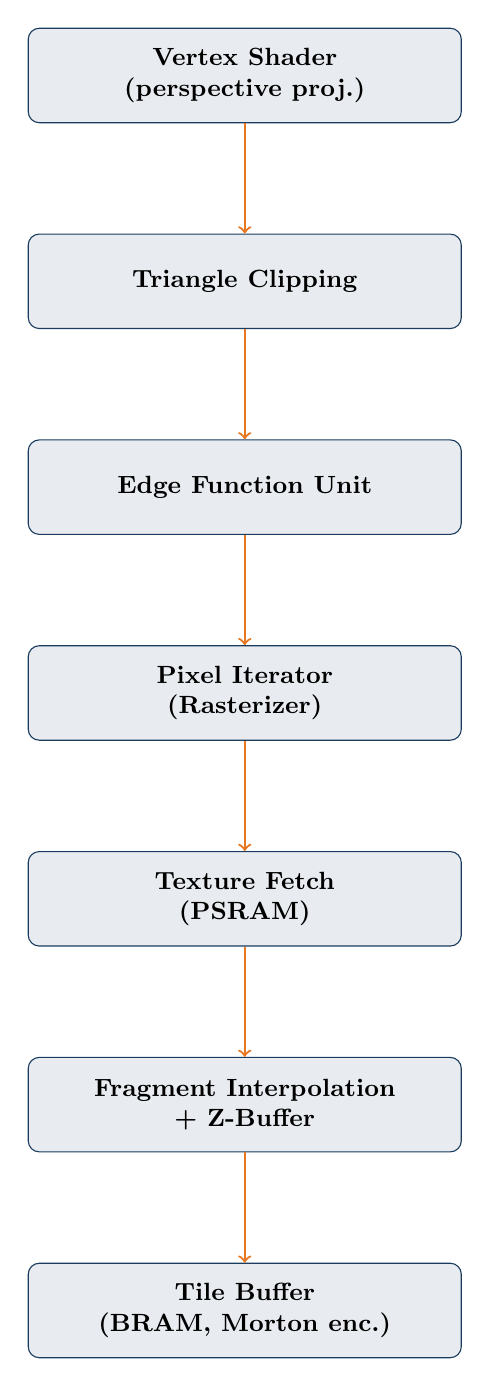
\begin{tikzpicture}[
  box/.style={draw=borgblue, fill=borgblue!10, rounded corners,
              minimum width=5.5cm, minimum height=1.2cm,
              font=\small\bfseries, align=center},
  arr/.style={->, thick, color=borgorange},
  node distance=1.4cm
]
\node[box] (vs)   {Vertex Shader\\(perspective proj.)};
\node[box] (clip) [below=of vs]  {Triangle Clipping};
\node[box] (ef)   [below=of clip]{Edge Function Unit};
\node[box] (ras)  [below=of ef]  {Pixel Iterator\\(Rasterizer)};
\node[box] (tex)  [below=of ras] {Texture Fetch\\(PSRAM)};
\node[box] (frag) [below=of tex] {Fragment Interpolation\\+ Z-Buffer};
\node[box] (tile) [below=of frag]{Tile Buffer\\(BRAM, Morton enc.)};
\draw[arr] (vs)--(clip); \draw[arr](clip)--(ef);
\draw[arr] (ef)--(ras);  \draw[arr](ras)--(tex);
\draw[arr] (tex)--(frag);\draw[arr](frag)--(tile);
\end{tikzpicture}
\end{center}

\medskip
Geometry is processed tile-by-tile; only \emph{visible} fragments are
shaded, minimising external memory bandwidth — critical for embedded
FPGAs with limited PSRAM bandwidth.
}

\column{0.25}

\block{Completed Pipeline (Steps 1–20)}{
All 20 steps completed in \textbf{28 days} (19 Mar – 14 Apr 2026):

\medskip
\begin{tabular}{@{}clr@{}}
\toprule
& \textbf{Component} & \textbf{Date} \\
\midrule
\done & Hardware Edge Function Unit       & 2026-03-19 \\
\done & Multiple Triangles (Firmware)     & 2026-03-20 \\
\done & 32-bit RISC-V Expansion           & 2026-03-23 \\
\done & Larger Register File + IMEM       & 2026-03-23 \\
\done & Perspective Projection (HW)       & 2026-03-24 \\
\done & Hardware RCP Unit                 & 2026-03-24 \\
\done & Triangle Clipping (HW)            & 2026-03-27 \\
\done & Hardware Fragment Interpolation   & 2026-03-27 \\
\done & Arcilator + Verilator simulation  & 2026-03-29 \\
\done & Pixel Iterator (HW Rasterizer)    & 2026-04-05 \\
\done & Hardware Z-Buffer Unit            & 2026-04-07 \\
\done & Command FIFO                      & 2026-04-08 \\
\done & SystemRDL Register Description    & 2026-04-08 \\
\done & Interactive Viewer                & 2026-04-10 \\
\done & Texture Fetch Unit                & 2026-04-13 \\
\done & LUT Recovery                      & 2026-04-13 \\
\done & SoC Project Restructure           & 2026-04-13 \\
\done & Shared Memory Controller          & 2026-04-14 \\
\done & IO Bundle Refactor                & 2026-04-14 \\
\bottomrule
\end{tabular}
}

\block{Current Demo}{
Running on \textbf{pico-ice} (iCE40 UP5K, 5280 LCs):
\begin{itemize}[leftmargin=*,nosep]
  \item 12 textured triangles, 32$\times$32 framebuffer
  \item Full pipeline: vertex shader $\to$ texture fetch $\to$ Z-buffer $\to$ output
  \item CPU-orchestrated (GPU autonomy = Phase 2, in progress)
\end{itemize}

\medskip
\textbf{Bandwidth note:} Current bottleneck is shared CPU/GPU PSRAM access.
GPU DMA engine (Step 22) will eliminate CPU involvement in rendering.
}

\column{0.25}

\block{FPGA Resource Budget (iCE40 UP5K)}{
\begin{center}
\begin{tabular}{@{}lrr@{}}
\toprule
\textbf{Resource} & \textbf{Used} & \textbf{Available} \\
\midrule
Logic Cells    & $\sim$5\,100  & 5\,280 \\
BRAMs (4 kb)   & $\sim$10     & 30 \\
DSPs           & 0            & 8 \\
\bottomrule
\end{tabular}
\end{center}

\medskip
Operating within a \$20 FPGA forces disciplined area optimisation:
nibble-serial FMAs, shared memory controllers,
and PeakRDL-generated register files contribute to fitting
a full GPU pipeline in 5\,280 logic cells.
}

\block{ASIC Tapeouts}{
\begin{tabular}{@{}llll@{}}
\toprule
\textbf{Run} & \textbf{Process} & \textbf{Content} & \textbf{Date} \\
\midrule
TTIHP26a & IHP SG13G2 130\,nm  & FP adder peripheral   & Mar 2026 \\
TTSKY26a & SkyWater SKY130     & Triangle rasteriser   & May 2026 \\
GF180    & GlobalFoundries 180\,nm& Diffuse shader ASIC & 2022 \\
\bottomrule
\end{tabular}

\medskip
All tapeouts via the \textbf{Tiny Tapeout} open-access silicon programme
and the \textbf{Google Open-Source Silicon Programme}.
Chips for TTIHP26a expected July 2026.
}

\block{Open-Source Toolchain}{
\begin{tabular}{@{}ll@{}}
\textbf{HDL}        & Chisel (Scala) $\to$ FIRRTL $\to$ Verilog \\
\textbf{Synthesis}  & Yosys \\
\textbf{P\&R FPGA}  & nextpnr-ice40 \\
\textbf{P\&R ASIC}  & OpenROAD / OpenLane \\
\textbf{Simulation} & Verilator, cocotb, Arcilator \\
\textbf{Reg. map}   & PeakRDL-chisel \\
\end{tabular}
}

\column{0.25}

\block{Comparison with Related Open-Source GPUs}{
\begin{tabular}{@{}lccc@{}}
\toprule
& \textbf{Borg} & \textbf{Nyuzi} & \textbf{Vortex} \\
\midrule
Architecture    & TBDR    & GPGPU   & RISC-V GPGPU \\
ISA             & Custom  & Custom  & RV32\\
Tapeout         & \done   & —       & — \\
Open toolchain  & \done   & partial & partial \\
FPGA target     & iCE40   & Arria~5 & Xilinx \\
Focus           & Graphics& Compute & Compute \\
\bottomrule
\end{tabular}
}

\block{Funding}{
\begin{center}

\includegraphics[height=2cm]{figures/nlnet_logo}
\qquad

\includegraphics[height=2cm]{figures/ngi0_logo}
\end{center}
\medskip
Borg is funded by the \textbf{NGI0 Commons Fund}, established by
NLnet Foundation with financial support from the European Commission's
Next Generation Internet programme
(Grant Agreement No.~101135429, DG~CONNECT),
and by the Swiss State Secretariat for Education, Research and Innovation (SERI).
}

\block{Future Work}{
\begin{itemize}[leftmargin=*,nosep]
  \item \inprog\ \textbf{GPU autonomy} (Steps 21–26): DMA engine, write port,
    integrated vertex sequencer, real-time VGA output
  \item ULX3S / ECP5 port for higher resolution
  \item ISA extensions for BVH ray traversal (path tracing on Borg)
  \item Integration with \textsc{Gonzales} path tracer:
    first fully open-source hardware path tracer
\end{itemize}
}

\block{References}{
\small
[1] Woop et al.\ \emph{RPU: A Programmable Ray Processing Unit}, SIGGRAPH 2005.\\
[2] Borg GPU book: \url{https://gonsolo.github.io/Borg}\\
[3] Source: \url{https://github.com/gonsolo/Borg}
}

\end{columns}

\end{document}
